\section{Anhang}
\label{sec:Anhang}
\begin{table}[H]
    \centering
    \caption{Messdaten zur Rechtecksschwingung.}
    \label{tab:Rechteck}
    \begin{tblr}{
        colspec = {c c || c c}
    }
        \toprule
        $\nu$ / kHz & $U$ / V & dB & $\nu$ / kHz & $U$ / V & dB\\
        \midrule
        10  &  89.12 & 39.0 & 210 &  4.26 & 12.6 \\
        30  &  29.51 & 29.4 & 230 &  3.89 & 11.8 \\
        50  &  17.78 & 25.0 & 250 &  3.54 & 11.0 \\
        70  &  12.30 & 21.8 & 270 &  3.23 & 10.2 \\
        90  &  9.77  & 19.8 & 290 &  3.16 & 10.0 \\
        110 &  8.12  & 18.2 & 310 &  2.95 & 9.41 \\
        130 &  6.76  & 16.6 & 330 &  2.82 & 9.01 \\
        150 &  5.88  & 15.4 & 350 &  2.69 & 8.61 \\
        170 &  5.37  & 14.6 & 370 &  2.45 & 7.81 \\
        190 &  4.67  & 13.4 & 390 &  2.45 & 7.81 \\
        \bottomrule
    \end{tblr}
\end{table}

\begin{table}[H]
    \centering
    \caption{Messdaten zur Dreiecksschwingung.}
    \label{tab:Dreieck}
    \begin{tblr}{colspec = {c c}}
         \toprule
        $\nu$ / kHz & dB & $U$ / V & dB\\
        \midrule
        10  & 56.23 & 35.0  \\
        30  & 6.30  & 16.0  \\
        50  & 2.24  & 7.01  \\
        70  & 1.14  & 1.21  \\
        90  & 0.67  & -3.39 \\
        110 & 0.46  & -6.59 \\
        \bottomrule
    \end{tblr}
\end{table}

\begin{table}[H]
    \centering
    \caption{Messdaten zur Sägezahnschwingung.}
    \label{tab:Sägezahn}
    \begin{tblr}{
        colspec = {c c c || c c c}
    }
        \toprule
        $\nu$ / kHz & $U$ / V & dB & $\nu$ / kHz & $U$ / V & dB\\
        \midrule
        10  &  44.66 & 33.0 & 110 &  4.07 & 12.2 \\
        20  &  22.38 & 27.0 & 120 &  3.89 & 11.8 \\
        30  &  14.79 & 23.4 & 130 &  3.54 & 11.0 \\
        40  &  11.22 & 21.0 & 140 &  3.31 & 10.4 \\
        50  &  8.91  & 19.0 & 150 &  3.09 & 9.81 \\
        60  &  7.41  & 17.4 & 160 &  2.82 & 9.01 \\
        70  &  6.45  & 16.2 & 170 &  2.69 & 8.61 \\
        80  &  5.62  & 15.0 & 180 &  2.57 & 8.21 \\
        90  &  4.89  & 13.8 & 190 &  2.45 & 7.81 \\
        100 &  4.46  & 13.0 &     &       &      \\
        \bottomrule
    \end{tblr}
\end{table}
\begin{figure}[H]
    \centering
    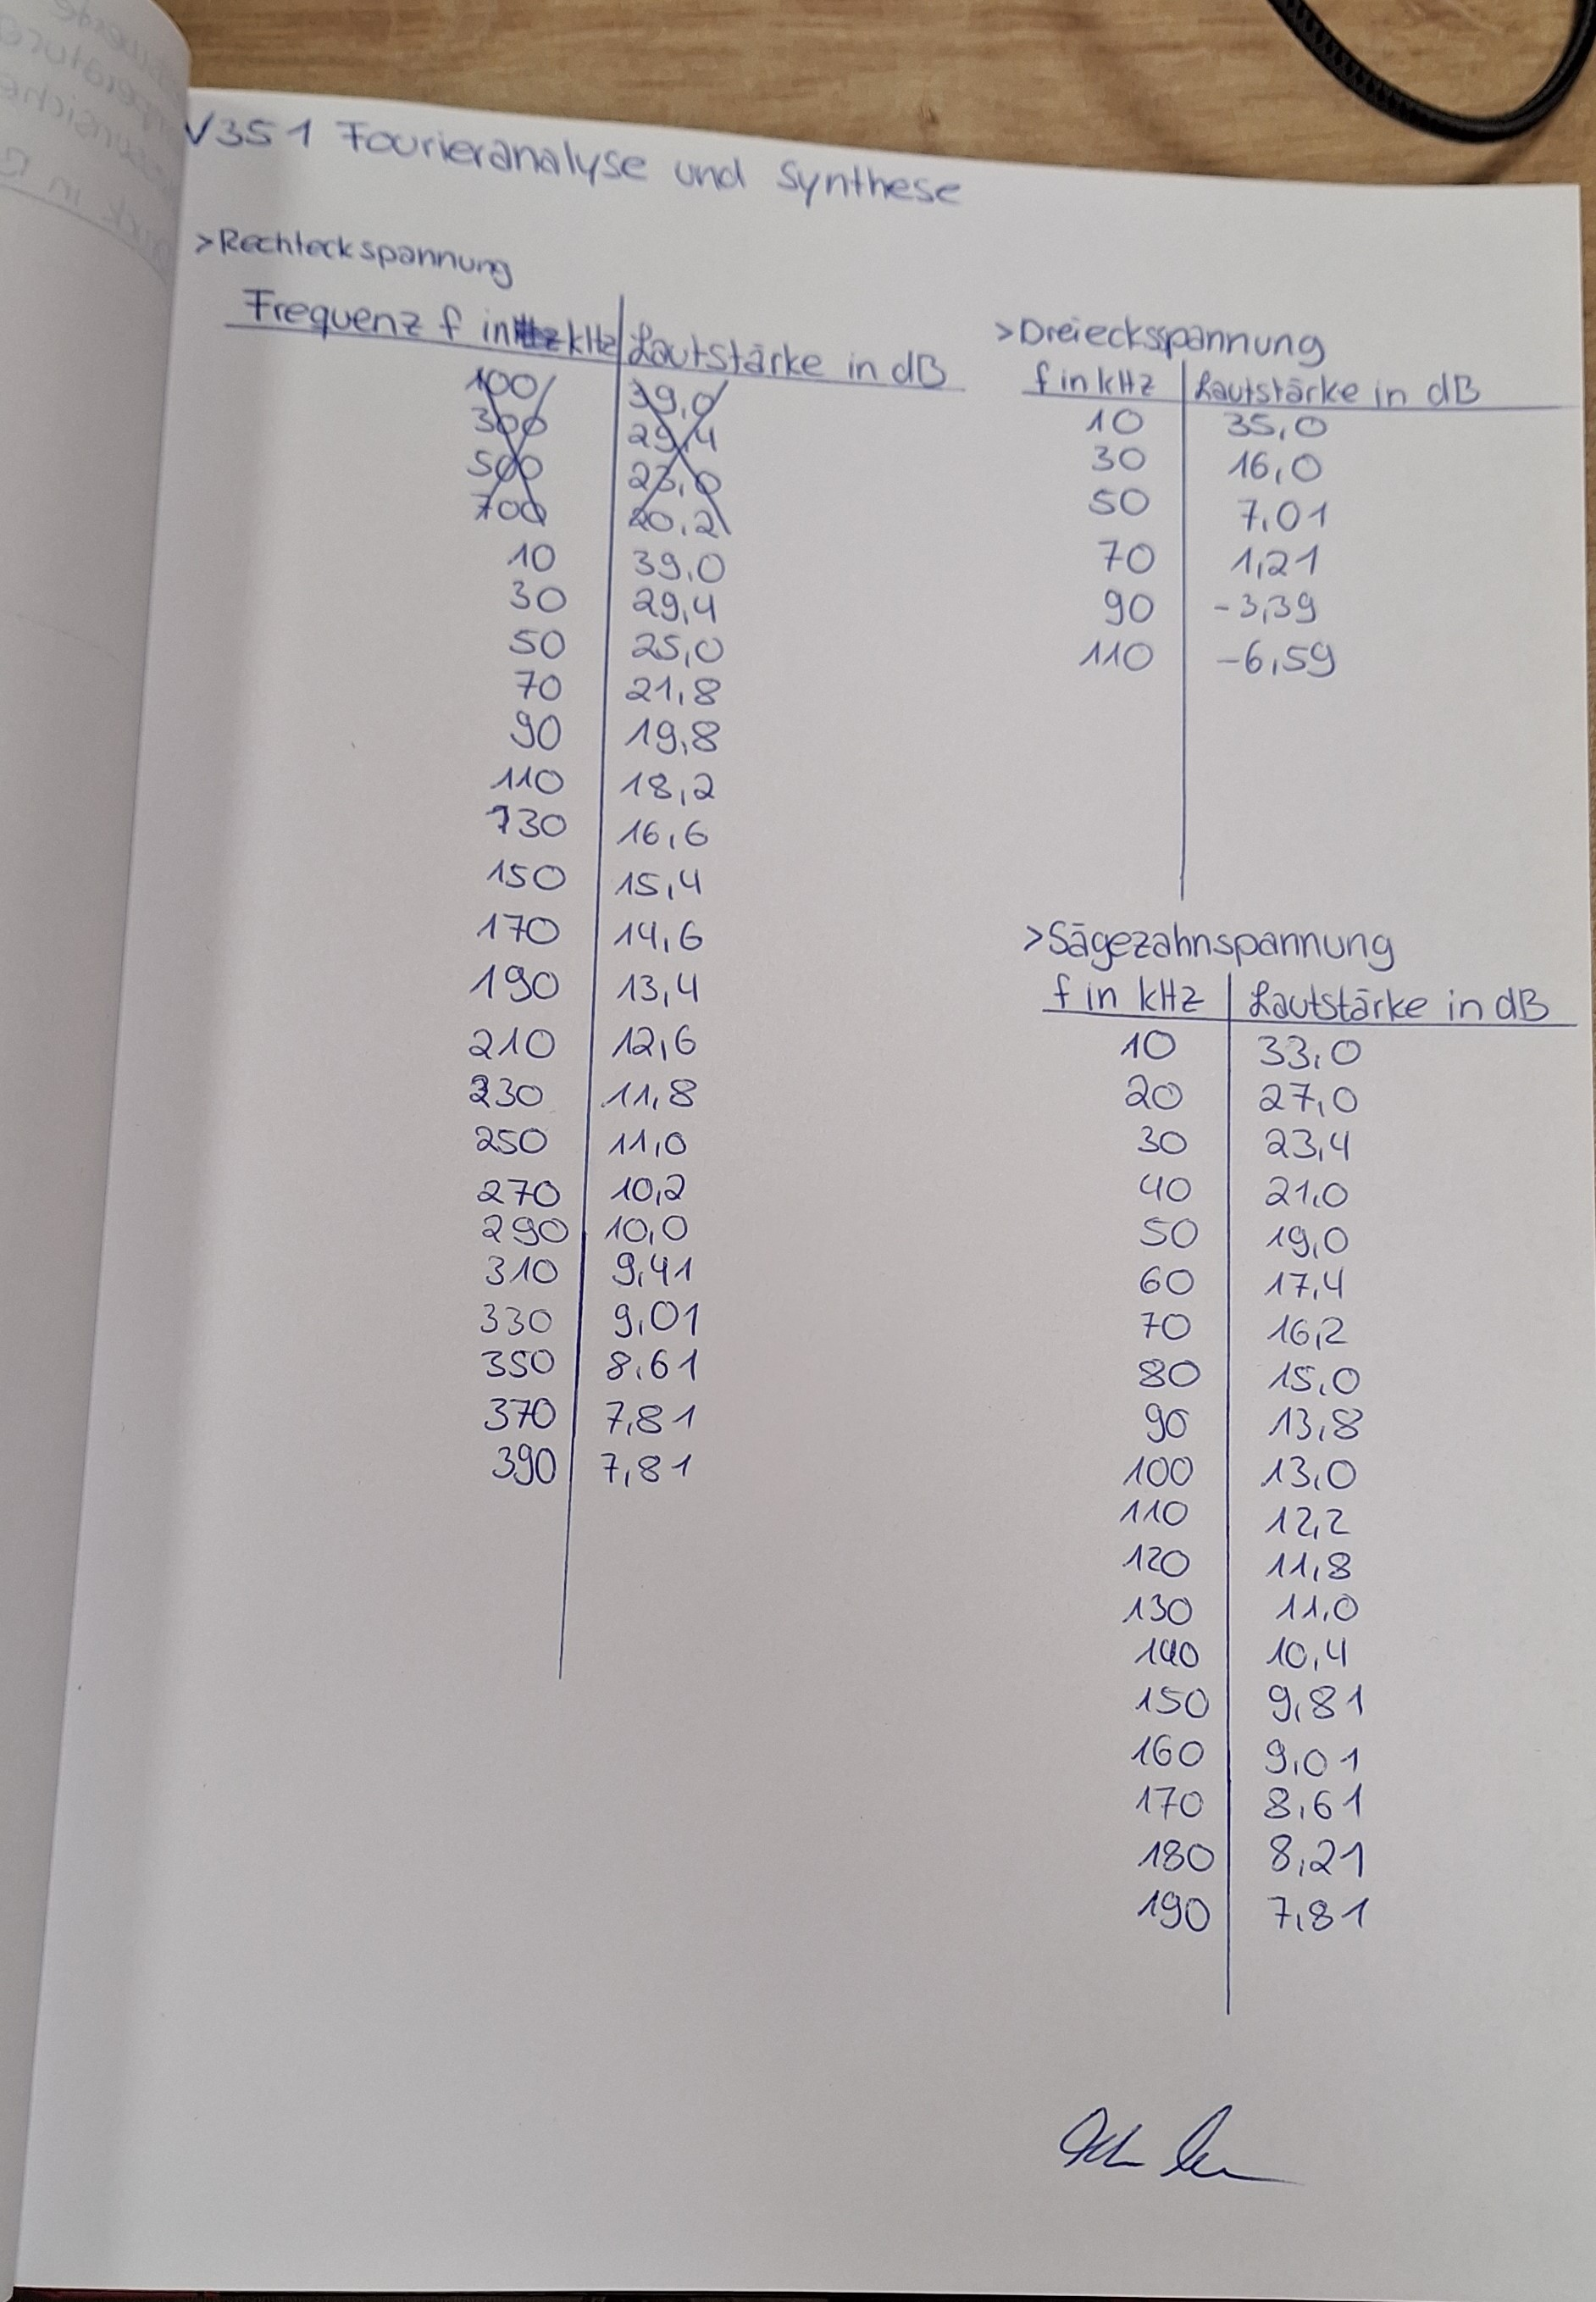
\includegraphics[width=\textwidth]{Messdaten_Bilder/Messdaten.jpg}
\end{figure} 